\documentclass[main.tex]{subfiles}


\begin{document}

\section{Simulation and Results}\label{sec:simulation}

This section aims to visualize the results obtained with the proposed method. In the following, there is first defined the trajectory used for the task reference. Then, there are shown plots, tables and simulations.
Before defining the trajectories implemented, let's denote with:
\begin{itemize}
    \item 0, when the foot is in contact with the surface
    \item -, when the foot is off contact with the surface
\end{itemize}
The trajectories are defined with respect to contact point, not time.


\subsection{Trajectory Generation}

\subsubsection{Still Task}
In this task the robot should not move at any instant of time and thus keeping the same initial position. 
The contact sequence used is reported in Table ~\ref{tab:cs_still} where the first row concerns the right foot and the second row the left foot.
\begin{table}[H]
\label{tab:cs_still}
\centering
\begin{tabular}{|c|c|l|}
\hline
\textbf{Task} & \textbf{N} & \textbf{Contact Sequence} \\
\hline
Still & 3 & 
\begin{tabular}[c]{@{}l@{}} 
0\,0\,0\ \\
0\,0\,0\ 
\end{tabular} \\
\hline
\end{tabular}
\caption{Contact sequence for still task}
\end{table}

The trajectory is simply defined as follows:
\begin{algorithm}[H]
\caption{Reference Trajectory Initialization and Update}
\begin{algorithmic}[1]
\State Initialize $X_{\text{ref}} \in \mathbb{R}^{28 \times (N+1)}$, $U_{\text{ref}} \in \mathbb{R}^{27 \times N}$
\State Set initial CoM state, feet positions and orientations in $X_{\text{ref}}$
\State $\text{time} \gets 0$, $\text{sig\_idx} \gets 0$

\For{$t = 0$ to $N-1$}
    \State Read contact states from $\sigma$
    \State Set phase duration and contact force gains $\lambda$
    \State Update $U_{\text{ref}}$ with phase duration and $\lambda$
    \State $\text{sig\_idx} \gets \text{sig\_idx} + 2$
\EndFor

\For{$t = 1$ to $N$}
    \State Set CoM velocity and feet step velocities as the initial state values (zeros)
    \State Update CoM and feet positions based on velocity and duration
    \State Update time and orientations in $X_{\text{ref}}$ as initial state
    \State $\text{sig\_idx} \gets \text{sig\_idx} + 2$
\EndFor

\State \Return $X_{\text{ref}}, U_{\text{ref}}$
\end{algorithmic}
\end{algorithm}


\subsubsection{Walking Task}
For the walking task, the trajectory used relies on the following concepts:
during the double-contact phases, in which both feet are on the ground, namely [0, 0], the COM does not move forward. Instead, it moves forward (along the X axis) only during single-support phases (a step), namely when right/left foot is lifting ([-, 0] or [0, -] respectively). Therefore if the preceding phase is a double support, the current phase COM keeps the same position as before, while if the preceding phase is of single support, the current phase COM has the previous position + some displacement; The Z (height) of each foot is always zero since at the beginning of each phase the feet are on the ground, while the X increases in an alternating manner depending on which foot was lifted in the previous phase. Also, the feet moves simulating a real walk, where the foot that is moving "surpasses" the one in contact, touching the ground beyond it, instead of positioning just next to the contact foot like before.
Lastly, each foot is interpolated in the intra-phase height position by following a parabolic profile that starts and arrives at the corresponding positions given by the phases solutions, instead of using the fixed inputs (zero-hold).
The contact sequence used is reported in Table ~\ref{tab:cs} where the first row concerns the right foot and the second row the left foot.
\begin{table}[H]
\label{tab:cs}
\centering
\begin{tabular}{|c|c|l|}
\hline
\textbf{Task} & \textbf{N} & \textbf{Contact Sequence} \\
\hline
Walk & 24 & 
\begin{tabular}[c]{@{}l@{}} 
0\,0\,0\,-\,0\,0\,0\,-\,0\,0\,0\,-\,0\,0\,0\,-\,0\,0\,0\,-\,0\ \\
0\,-\,0\,0\,0\,-\,0\,0\,0\,-\,0\,0\,0\,-\,0\,0\,0\,-\,0\,0\,0 
\end{tabular} \\
\hline
\end{tabular}
\caption{Contact sequence for walking task}
\end{table}
The algorithm used for this task is shown below:


\begin{algorithm}
\caption{Reference Trajectory Initialization and Update}
\begin{algorithmic}[1]
\State Initialize $X_{\text{ref}} \in \mathbb{R}^{28 \times (N+1)}$, $U_{\text{ref}} \in \mathbb{R}^{27 \times N}$
\State Set initial CoM state, feet positions and orientations in $X_{\text{ref}}$
\State $\text{time} \gets 0$, $\text{sig\_idx} \gets 0$

\For{$t = 0$ to $N-1$}
    \State Read contact states from $\sigma$
    \State Set phase duration and contact force gains $\lambda$
    \State Update $U_{\text{ref}}$ with phase duration and $\lambda$
    \State $\text{sig\_idx} \gets \text{sig\_idx} + 2$
\EndFor

\For{$t = 1$ to $N$}
    \State Read current and previous contact states
    \State Set CoM velocity $(v_x, v_y)$ and feet step velocities
    \State Update CoM and feet positions based on velocity and duration
    \State Update time and orientations in $X_{\text{ref}}$
    \State $\text{sig\_idx} \gets \text{sig\_idx} + 2$
\EndFor

\State \Return $X_{\text{ref}}, U_{\text{ref}}$
\end{algorithmic}
\end{algorithm}


\subsection{Solutions}
Solutions of those problems and tasks are tuples (X, U) where X is the state vector with dimension N , and U is the input vector with dimension N-1.
\\The solution is computed with ipopt solver from Casadi optimizer. Both the reference and solution are contact-dependent, meaning that X and U contain values for each contact phase, thus to find the time dependent solution we used the dynamics. 

\subsection{Still Task: results}
In this case the state vector has dimension 3, and the input vector has dimension 2.
\subsubsection{CoM Plots}
The following plots report the CoM trajectory in time. 
The alternation between light and dark grey on the background suggests the switch between phases.
As plots suggest there's no significant motion in any direction.
\begin{figure}[H]
    \centering
    \begin{subfigure}[b]{0.45\textwidth}
        \centering
        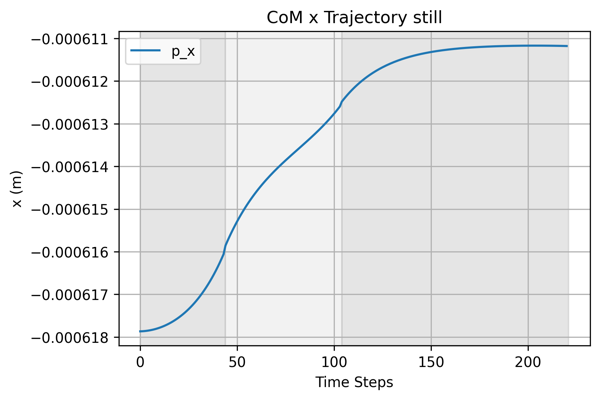
\includegraphics[width=\textwidth]{figures/CoM x Trajectory still.png}
        \caption{Com X Trajectory 1}
        \label{fig:sub1_still}
    \end{subfigure}
    \hfill
    \begin{subfigure}[b]{0.45\textwidth}
        \centering
        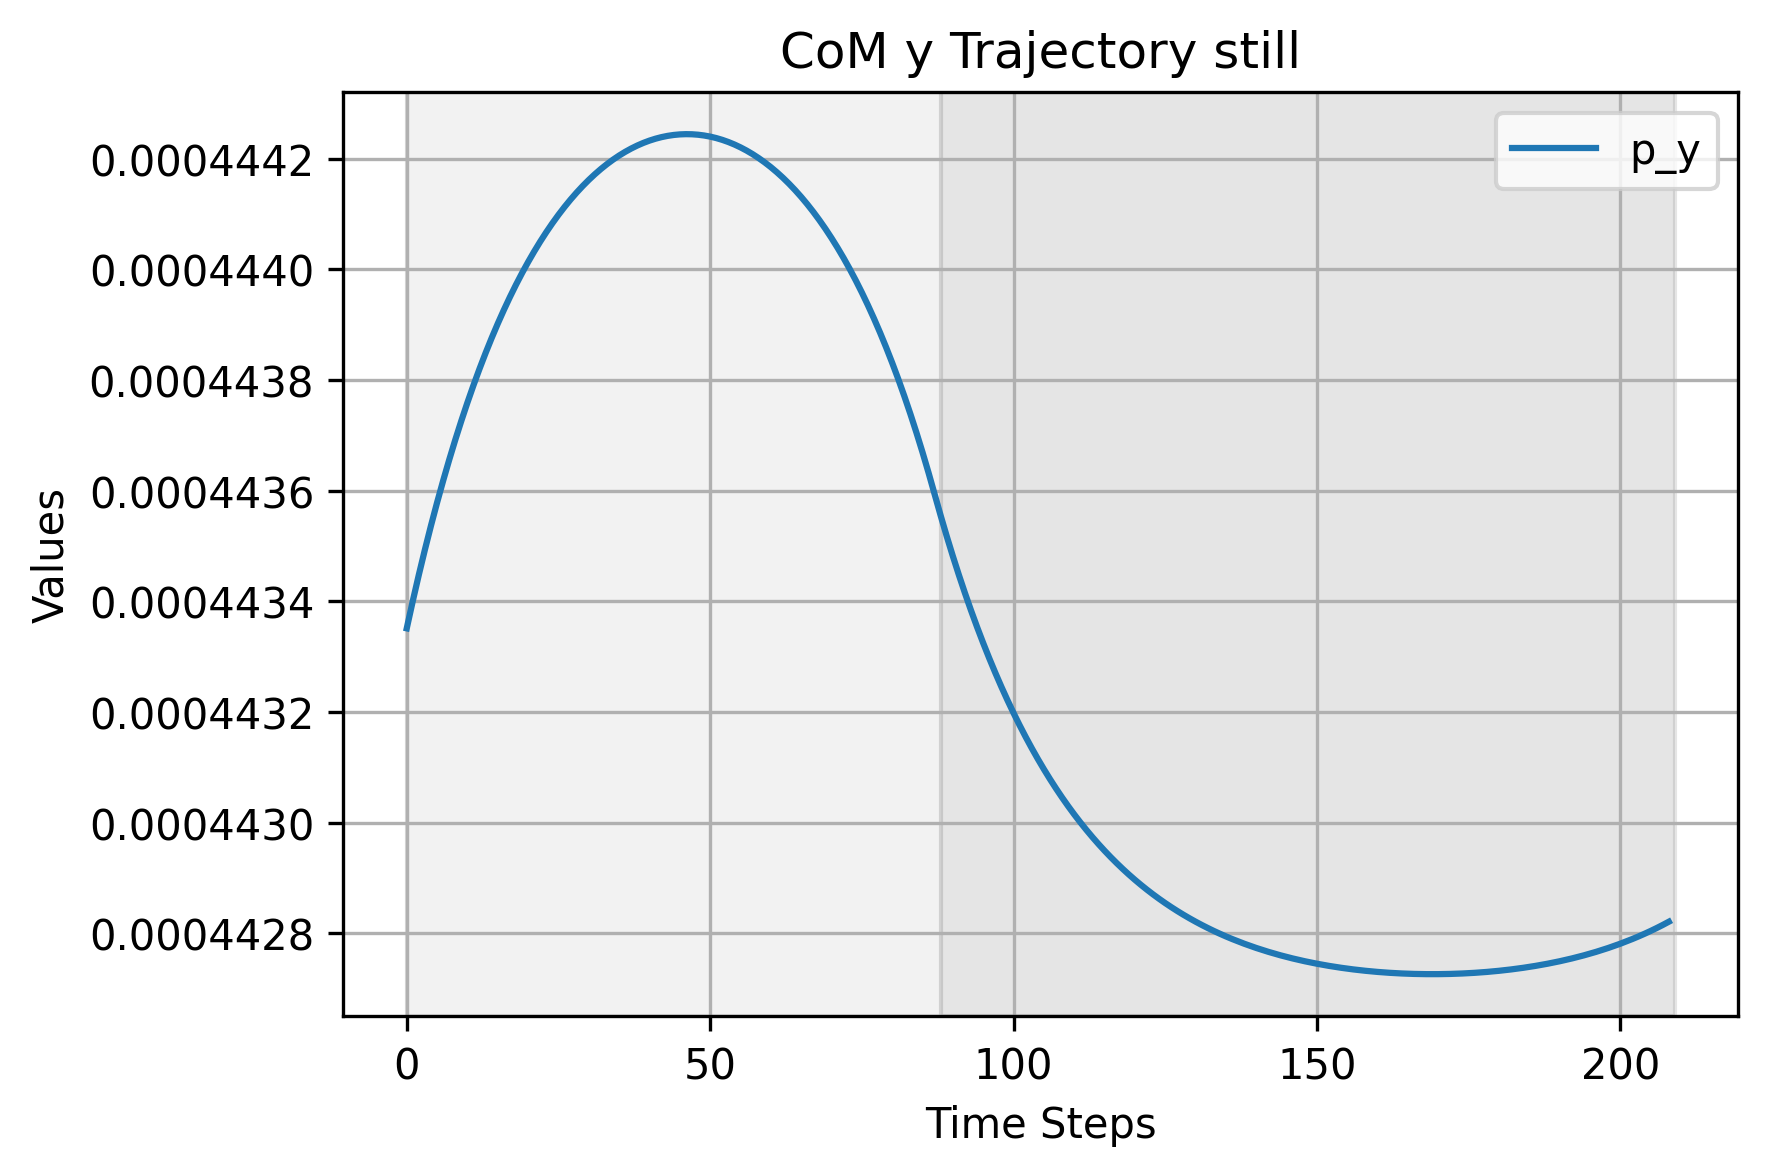
\includegraphics[width=\textwidth]{figures/CoM y Trajectory still.png}
        \caption{Com Y Trajectory 1}
        \label{fig:sub2_still}
    \end{subfigure}
    \hfill
    \begin{subfigure}[b]{0.45\textwidth}
        \centering
        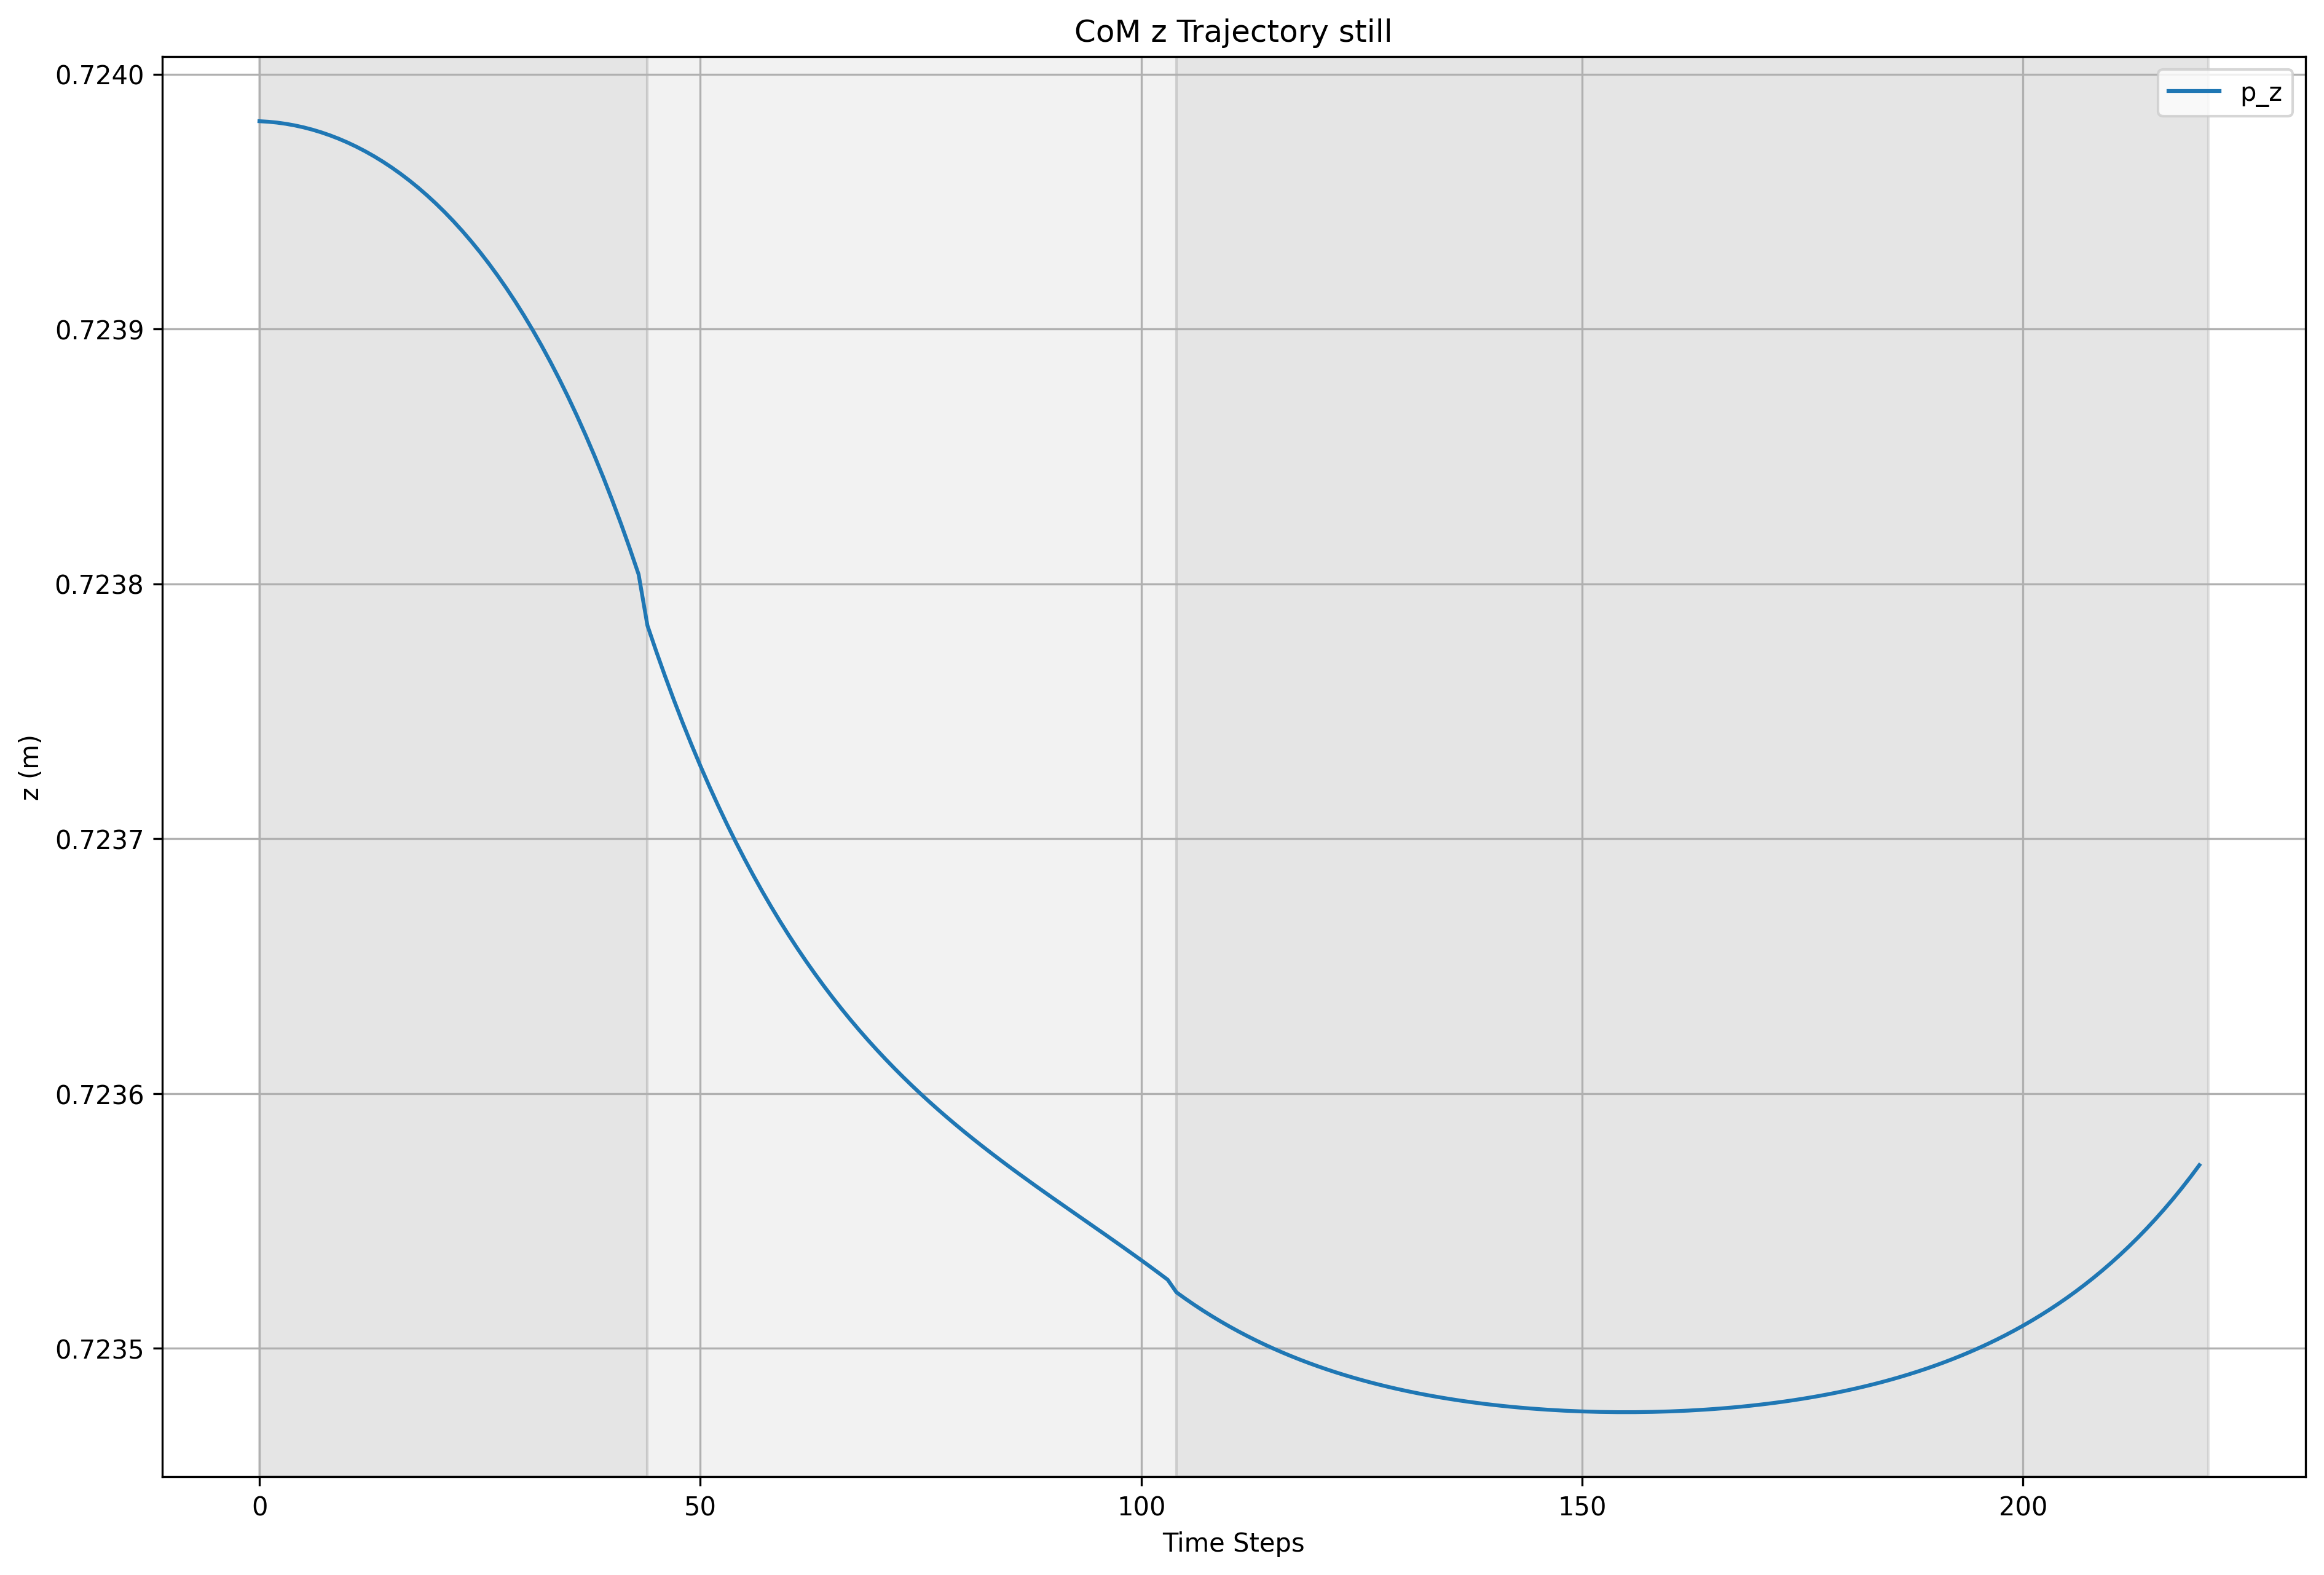
\includegraphics[width=\textwidth]{figures/CoM z Trajectory still.png}
        \caption{Com Z Trajectory 1}
        \label{fig:sub3_still}
    \end{subfigure}
    \caption{Com Trajectory}
    \label{fig:threeimages_still}
\end{figure}

\begin{figure}[htbp]
    \centering
    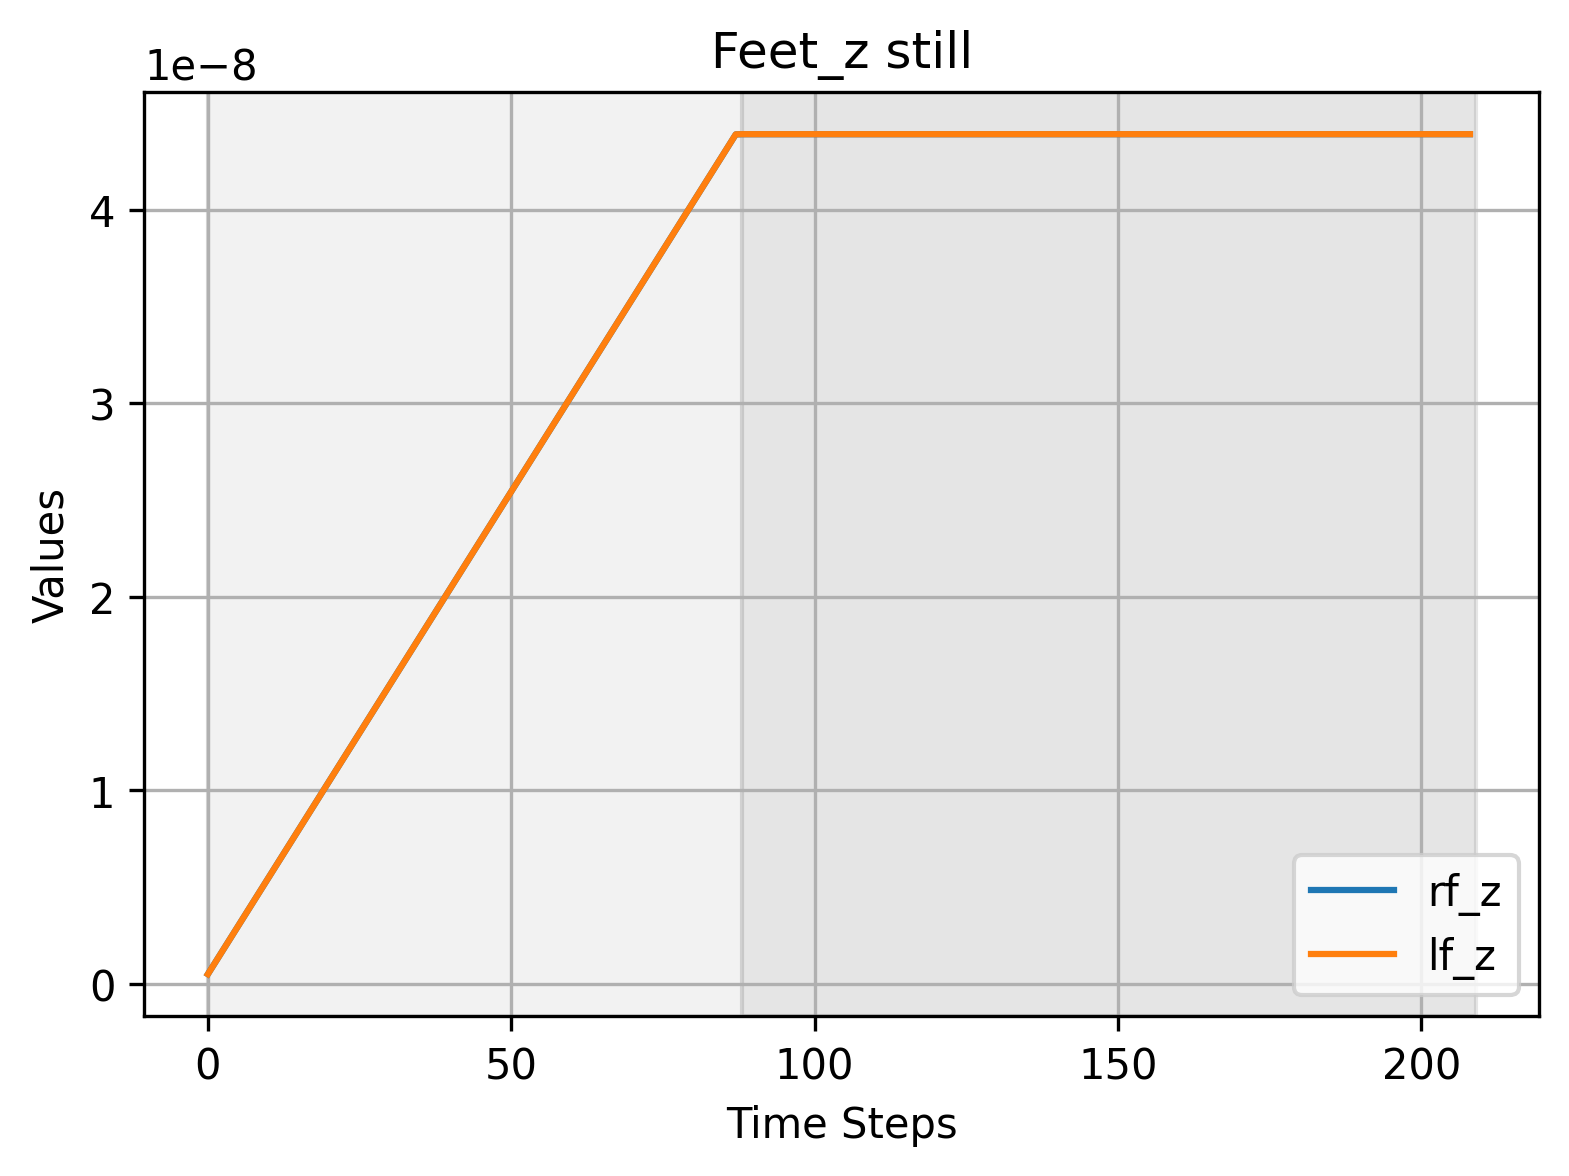
\includegraphics[width=0.6\textwidth]{figures/Feet_z still.png}
    \caption{Feet along Z}
    \label{fig:feet_still}
\end{figure}


\subsubsection{State and Input Contact Values}
In the following plots, the main components of the state and input vectors solutions are compared with the reference at each contact step.
\begin{figure}[htbp]
    \centering
    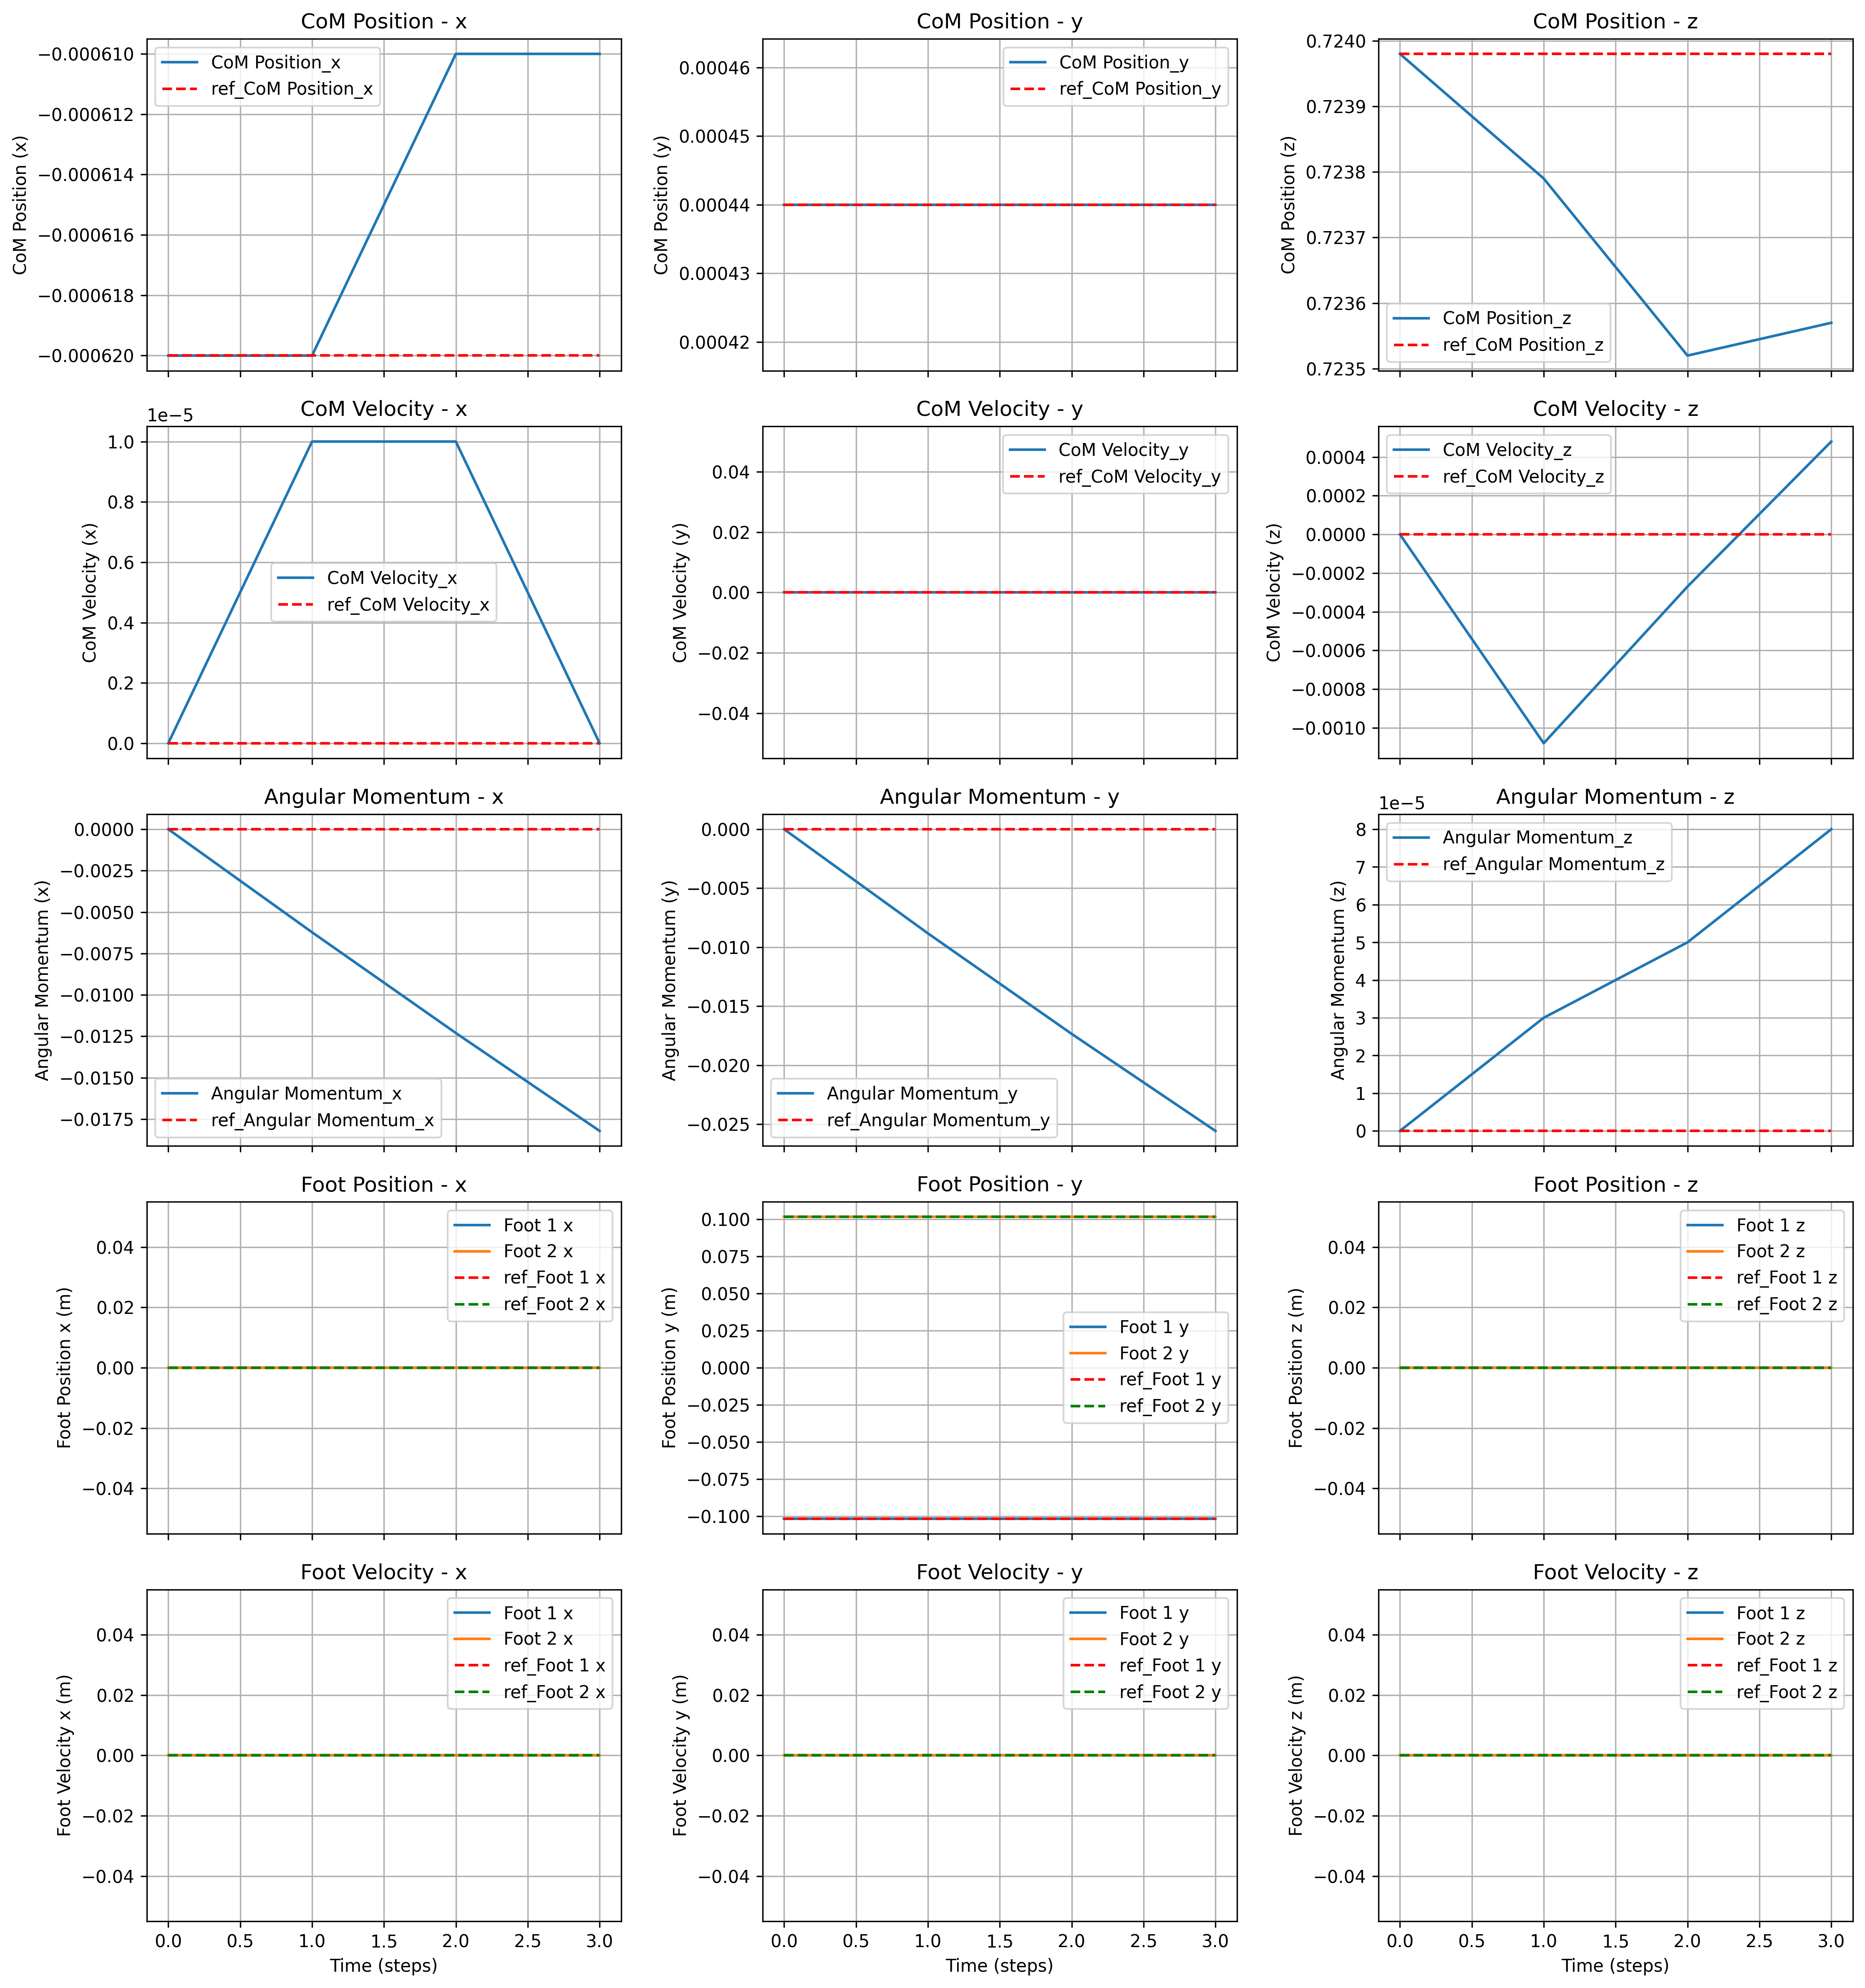
\includegraphics[width=0.6\textwidth]{figures/contact_x_still.png}
    \caption{Trajectory vs Reference: state vector}
    \label{fig:contact_x_still}
\end{figure}

\subsubsection{Contact Forces}
Another important dynamic aspect regards forces. 
In the input vector, the contact wrench that describes all the mechanical influence that a contact point (like a foot or hand) exerts on the robot or vice versa.
To balance dynamic laws, along the Z-axis the environment should exert a reaction force equal to the gravity factor multiplied by the mass of the robot. In the table ~\ref{tab:contact_forces_still}  below there are listed the contact forces exerting from the environment to both feet. As the table shows, when both feet are on the ground the gravity force is equally distributed on left and right foot.
\begin{table}[H]
\label{tab:contact_forces_still}
\centering
\begin{tabular}{ccc}
\toprule
Right Foot Z & Left Foot Z & $\Sigma_L^k$ \\
\midrule
49.0644 & 49.0531 & [0., 0.] \\
48.8973 & 49.65 & [0., 0.] \\
\bottomrule
\end{tabular}
\caption{Z-axis gravity force and $\Sigma_L^k$ values}
\end{table}

Components of contact wrench, rotational and translational forces, are graphically expressed in the following plots:
\begin{figure}[htbp]
    \centering
    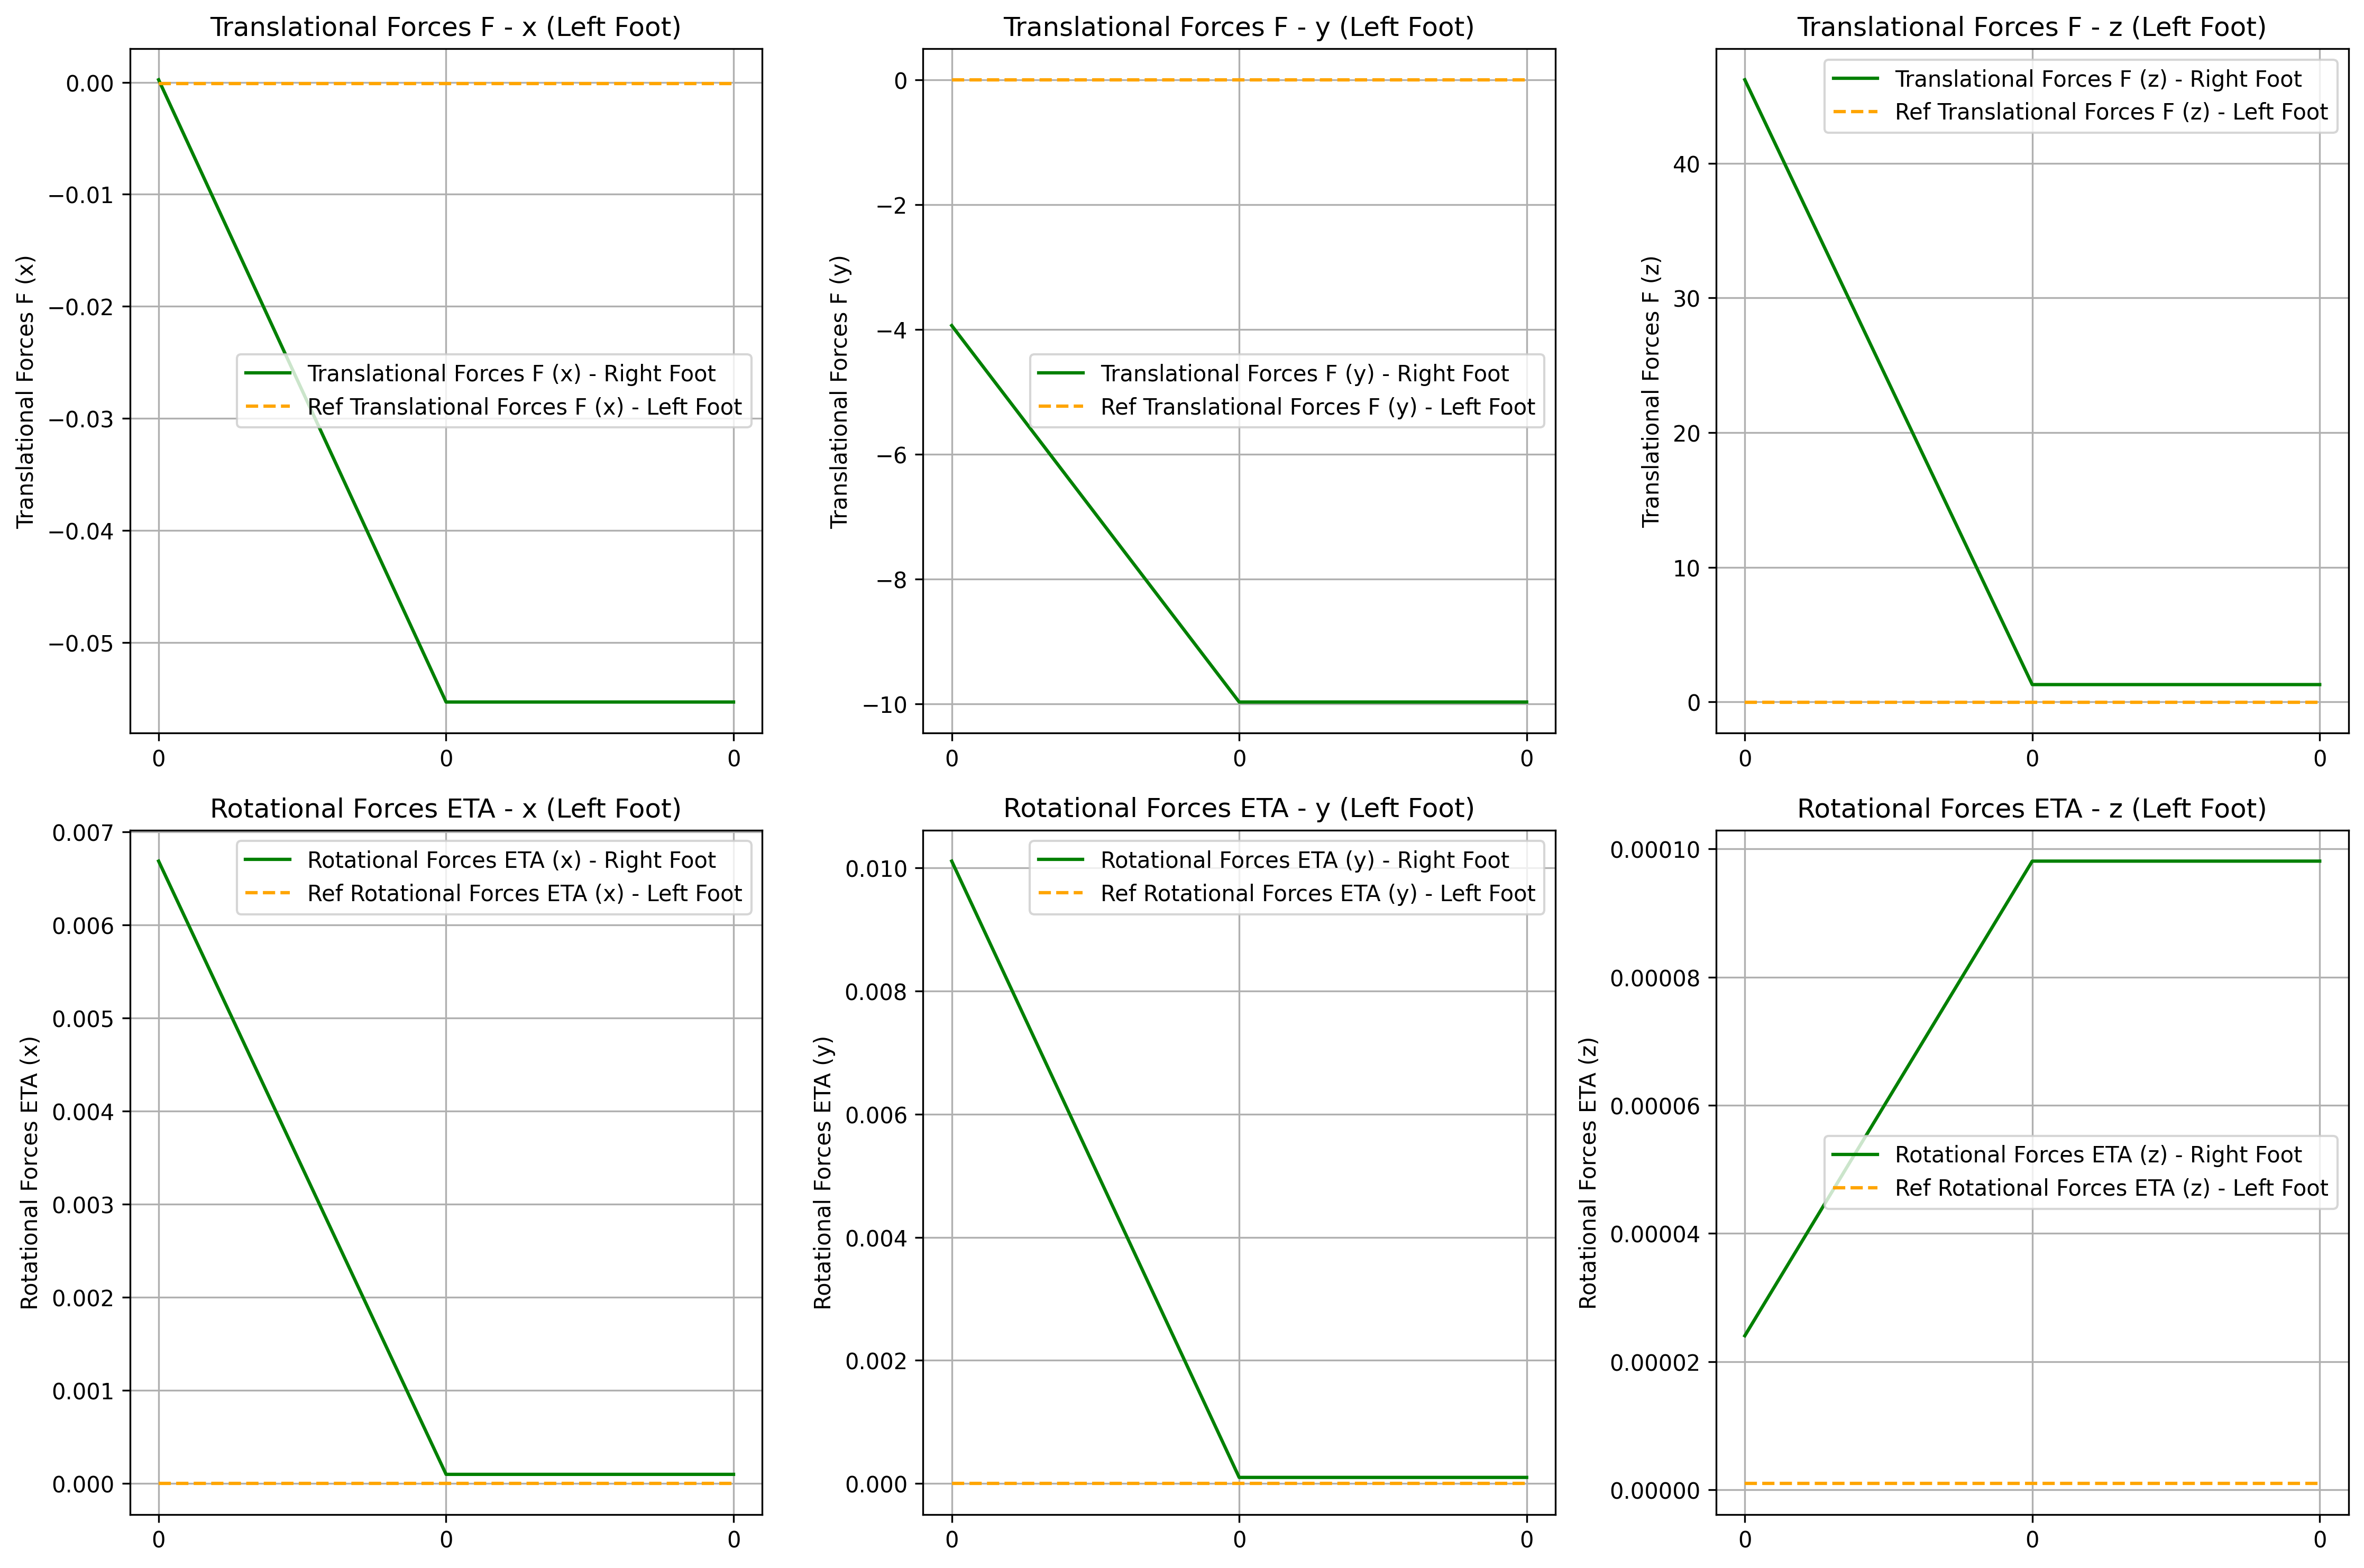
\includegraphics[width=0.8\textwidth]{figures/contact_forces_still.png}
    \caption{Trajectory vs Reference: Forces}
    \label{fig:contact_forces_still}
\end{figure}

\newpage
\subsubsection{Robot representation}
In this section it is possible to visualize first the path followed by the CoM, right and left foot in time:
\begin{figure}[htbp]
    \centering
    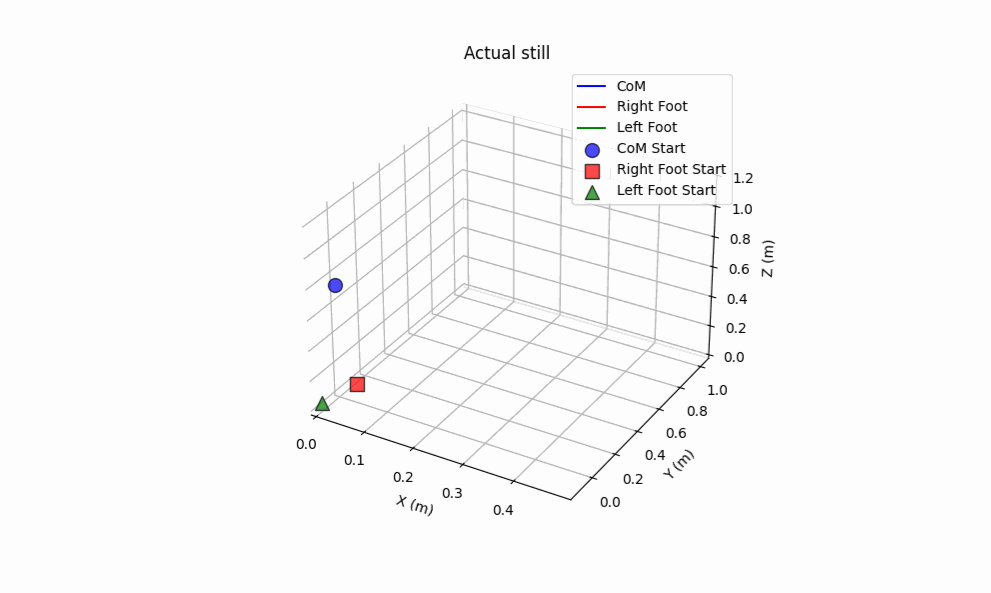
\includegraphics[width=0.8\textwidth]{figures/still.PNG}
    \caption{Still}
    \label{fig:still}
\end{figure}


\subsection{Walking Task: results}
In this case the state vector has dimension 24 and the input vector has dimension 23.


\subsubsection{CoM Plots}
The following plots report the CoM trajectory in time. 
The alternation between light and dark grey on the background suggests the switch between phases.
As Fig. ~\ref{fig:sub1} shows, the CoM exhibits linear motion in the x-direction.
Along the y-axis ~\ref{fig:sub2} the CoM goes towards the foot staying on the ground when lifting the other. Let's consider the first two contacts: in the first one, the robot is in double support (both feet are on the ground), while the second one expects the left foot to raise. Infact, the CoM at the end of the first phase has moved towards the right foot. This mechanism is repeated through all the alternances between double support and single support.
In the z-direction ~\ref{fig:sub3}, the CoM goes up and down in a small range of motion.
\begin{figure}[H]
    \centering
    \begin{subfigure}[b]{0.45\textwidth}
        \centering
        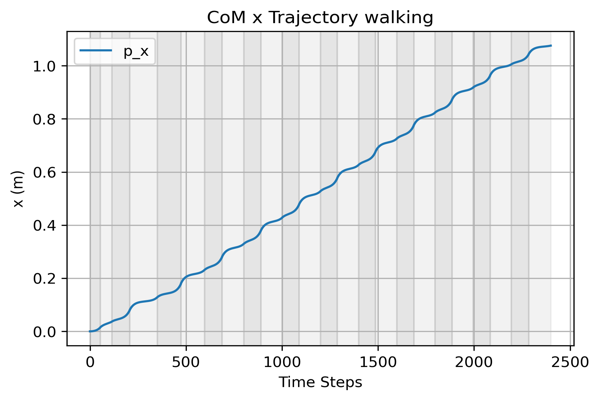
\includegraphics[width=\textwidth]{figures/CoM x Trajectory walking.png}
        \caption{Com X Trajectory 1}
        \label{fig:sub1_walking}
    \end{subfigure}
    \hfill
    \begin{subfigure}[b]{0.45\textwidth}
        \centering
        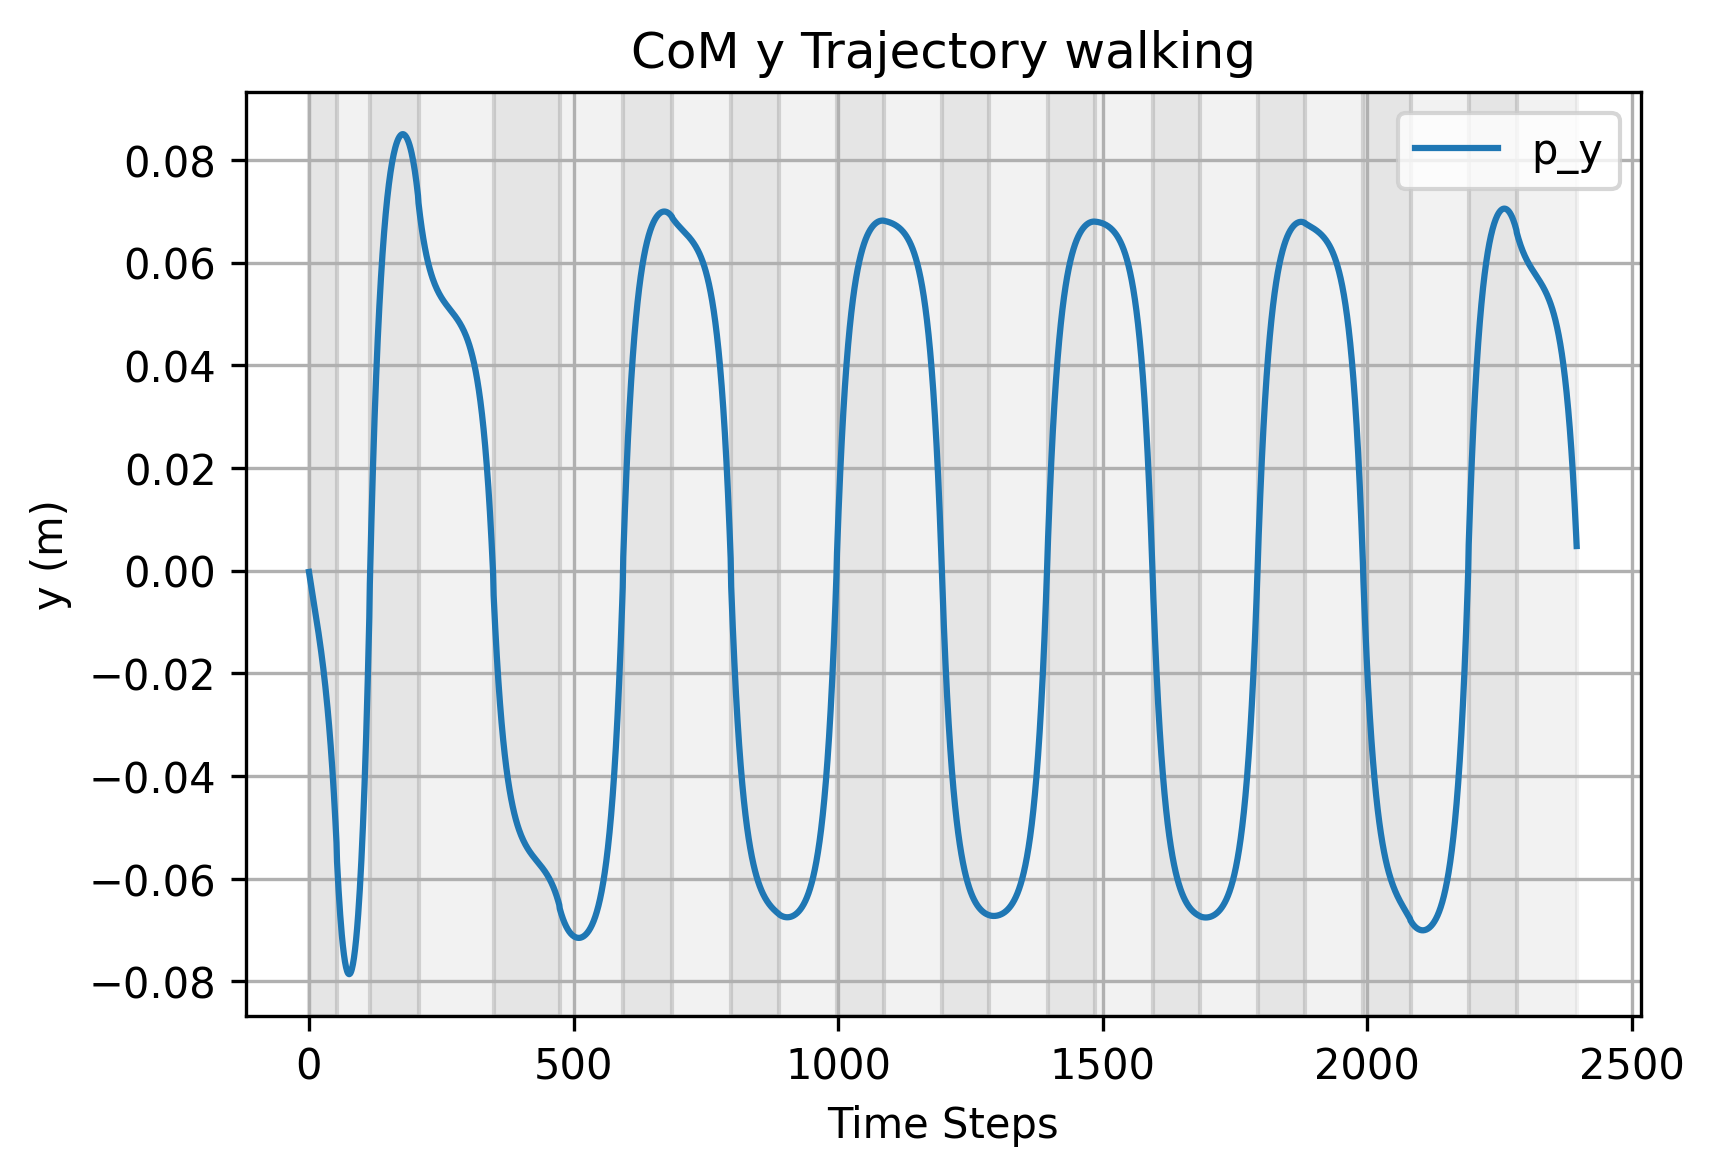
\includegraphics[width=\textwidth]{figures/CoM y Trajectory walking.png}
        \caption{Com Y Trajectory 1}
        \label{fig:sub2_walking}
    \end{subfigure}
    \hfill
    \begin{subfigure}[b]{0.45\textwidth}
        \centering
        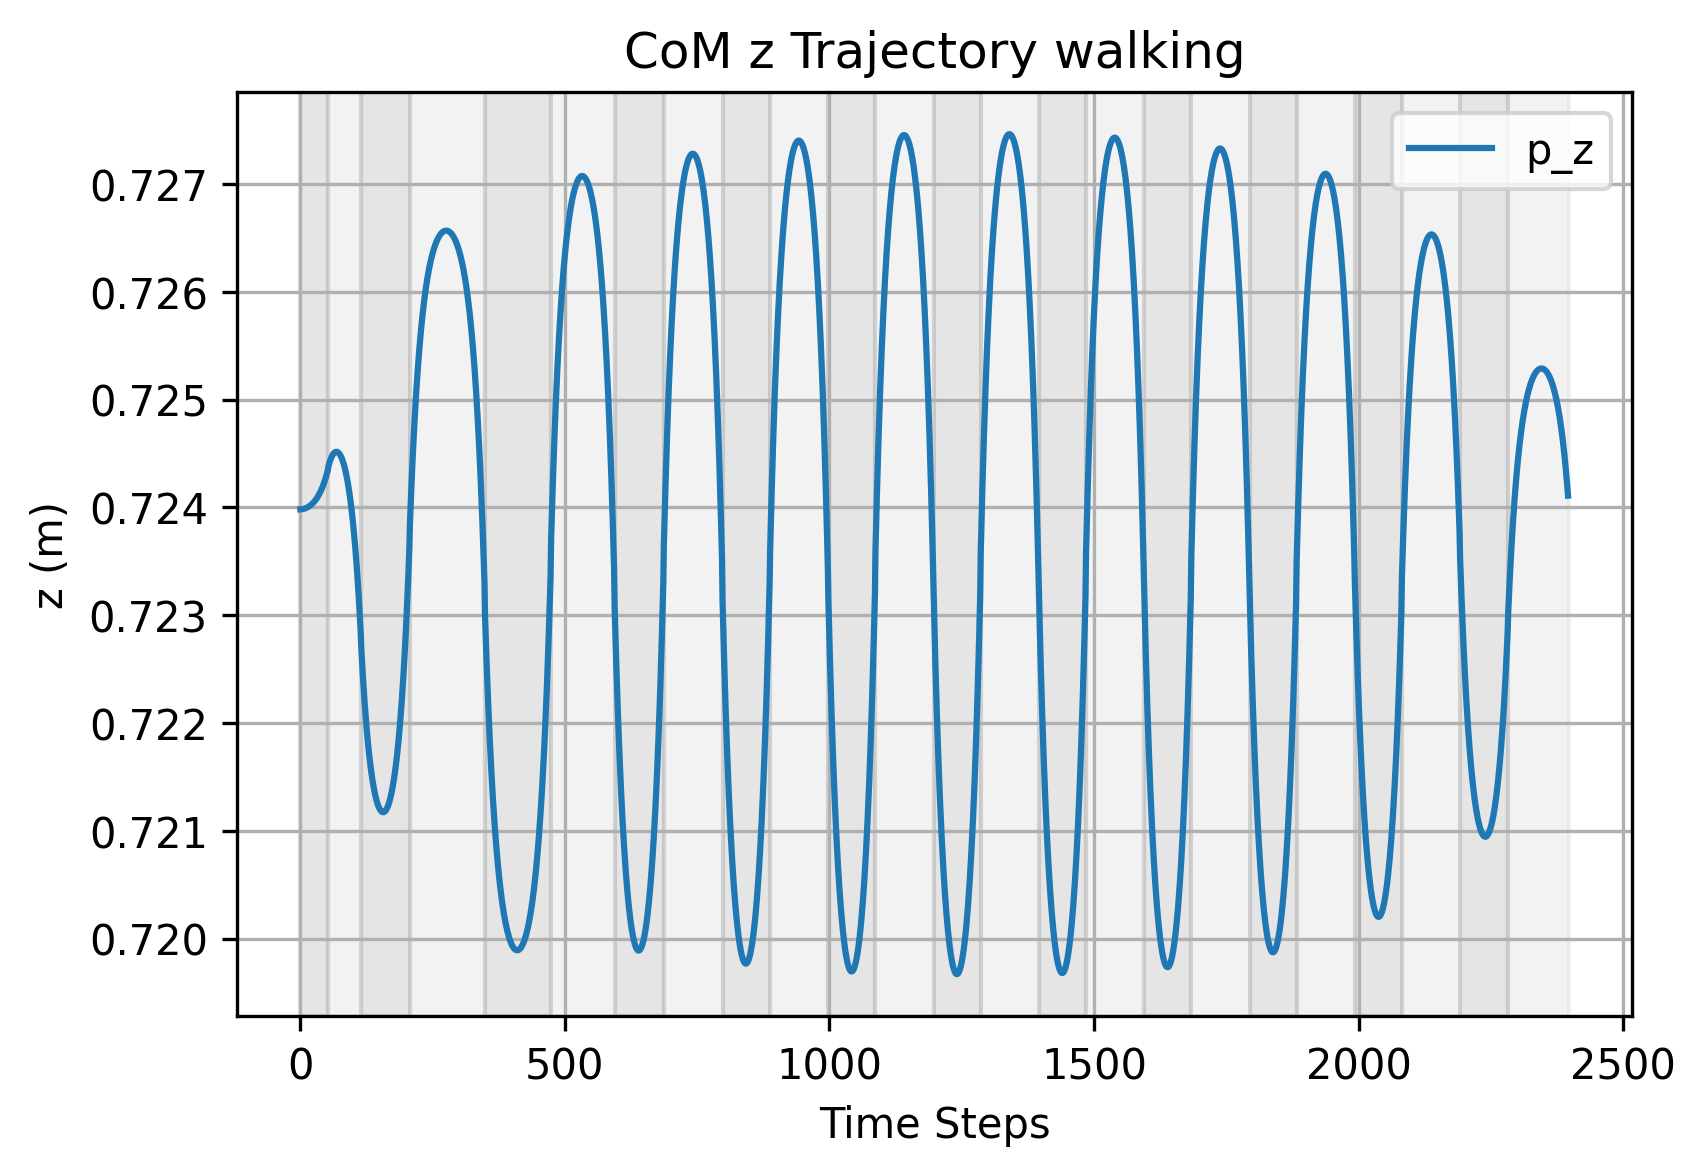
\includegraphics[width=\textwidth]{figures/CoM z Trajectory walking.png}
        \caption{Com Z Trajectory 1}
        \label{fig:sub3_walking}
    \end{subfigure}
    \caption{Com Trajectory}
    \label{fig:threeimages_walking}
\end{figure}
Furthermore, the image below represent the foot position along the Z-axis in time. As one can see, they follow a parabolic profile.  
\begin{figure}[htbp]
    \centering
    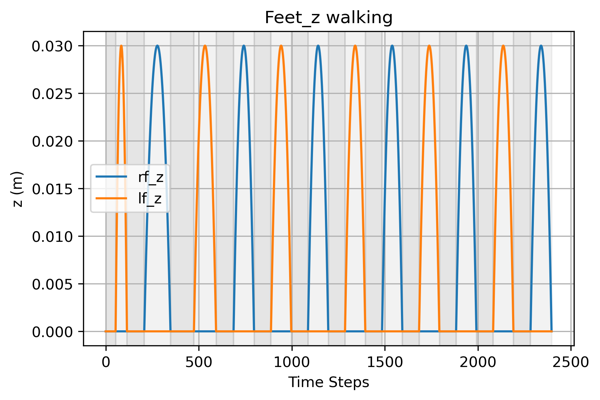
\includegraphics[width=0.6\textwidth]{figures/Feet_z walking.png}
    \caption{Feet along Z}
    \label{fig:feet_walking}
\end{figure}


\subsubsection{State and Input Contact Values}
In the following plots, the main components of the state and input vectors solutions are compared with the reference at each contact step.
\begin{figure}[htbp]
    \centering
    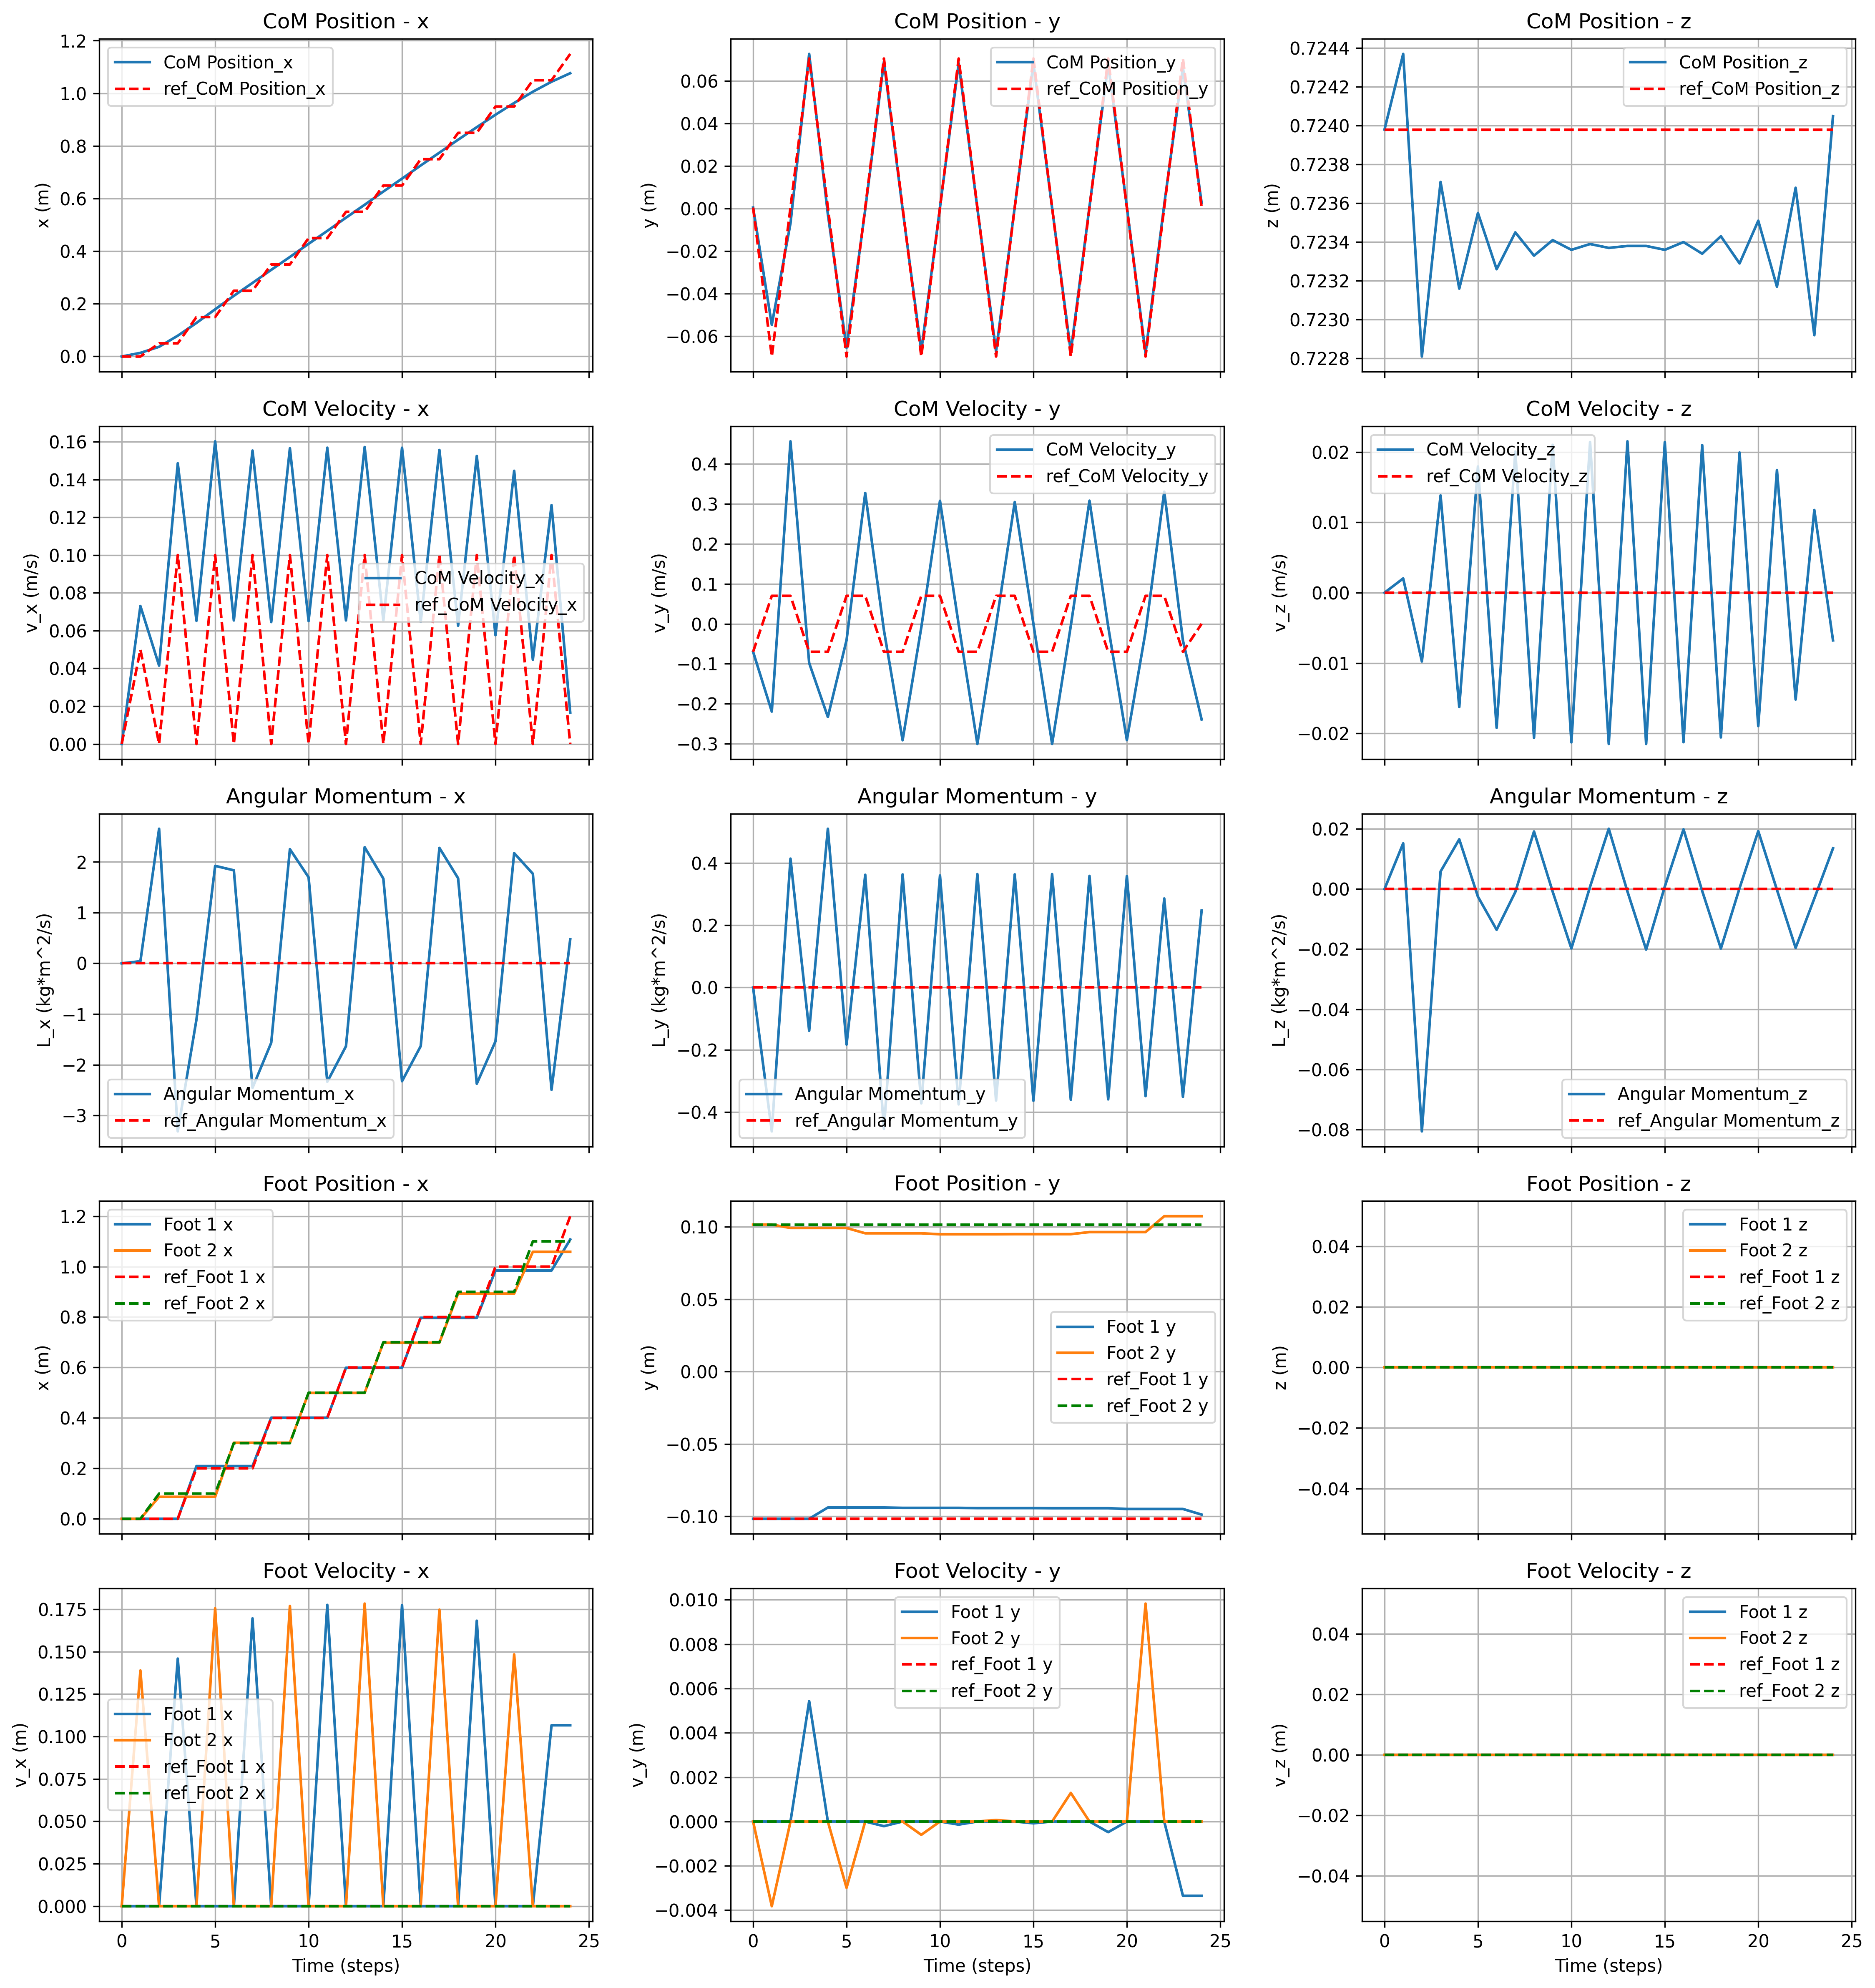
\includegraphics[width=0.6\textwidth]{figures/contact_x_walking.png}
    \caption{Trajectory vs Reference: state vector}
    \label{fig:contact_x_walking}
\end{figure}

\subsubsection{Contact Forces}
Another important dynamic aspect regards forces. 
In the input vector, the contact wrench that describes all the mechanical influence that a contact point (like a foot or hand) exerts on the robot or vice versa.
To balance dynamic laws, along the Z-axis the environment should exert a reaction force equal to the gravity factor multiplied by the mass of the robot. In the table ~\ref{tab:contact_forces_walking}  below there are listed the contact forces exerting from the environment to both feet. As the table shows, when both feet are on the ground the gravity force is equally distributed on left and right foot, while when one foot lifts the gravity force acts only on the foot staying on the ground.
\begin{table}[H]
\label{tab:contact_forces_walking}
\centering
\begin{tabular}{ccc}
\toprule
Right Foot Z & Left Foot Z & $\Sigma_L^k$ \\
\midrule
49.0644 & 49.0531 & [0., 0.] \\
97.9551 & 0 & [0., -] \\
48.8973 & 49.65 & [0., 0.] \\
0 & 97.4904 & [-, 0.] \\
49.6528 & 49.1563 & [0., 0.] \\
97.3081 & 0 & [0., -] \\
49.2399 & 49.7241 & [0., 0.] \\
0 & 97.2091 & [-, 0.] \\
49.7388 & 49.293 & [0., 0.] \\
97.1669 & 0 & [0., -] \\
49.3007 & 49.7613 & [0., 0.] \\
0 & 97.1486 & [-, 0.] \\
49.762 & 49.31 & [0., 0.] \\
97.1443 & 0 & [0., -] \\
49.3062 & 49.7655 & [0., 0.] \\
0 & 97.1495 & [-, 0.] \\
49.7557 & 49.3045 & [0., 0.] \\
97.1685 & 0 & [0., -] \\
49.2815 & 49.7467 & [0., 0.] \\
0 & 97.216 & [-, 0.] \\
49.7003 & 49.254 & [0., 0.] \\
97.3264 & 0 & [0., -] \\
49.1286 & 49.6485 & [0., 0.] \\
0 & 97.5828 & [-, 0.] \\
\bottomrule
\end{tabular}
\caption{Z-axis gravity force and $\Sigma_L^k$ values}
\end{table}

Components of contact wrench, rotational and translational forces, are graphically expressed in the following plots:
\begin{figure}[htbp]
    \centering
    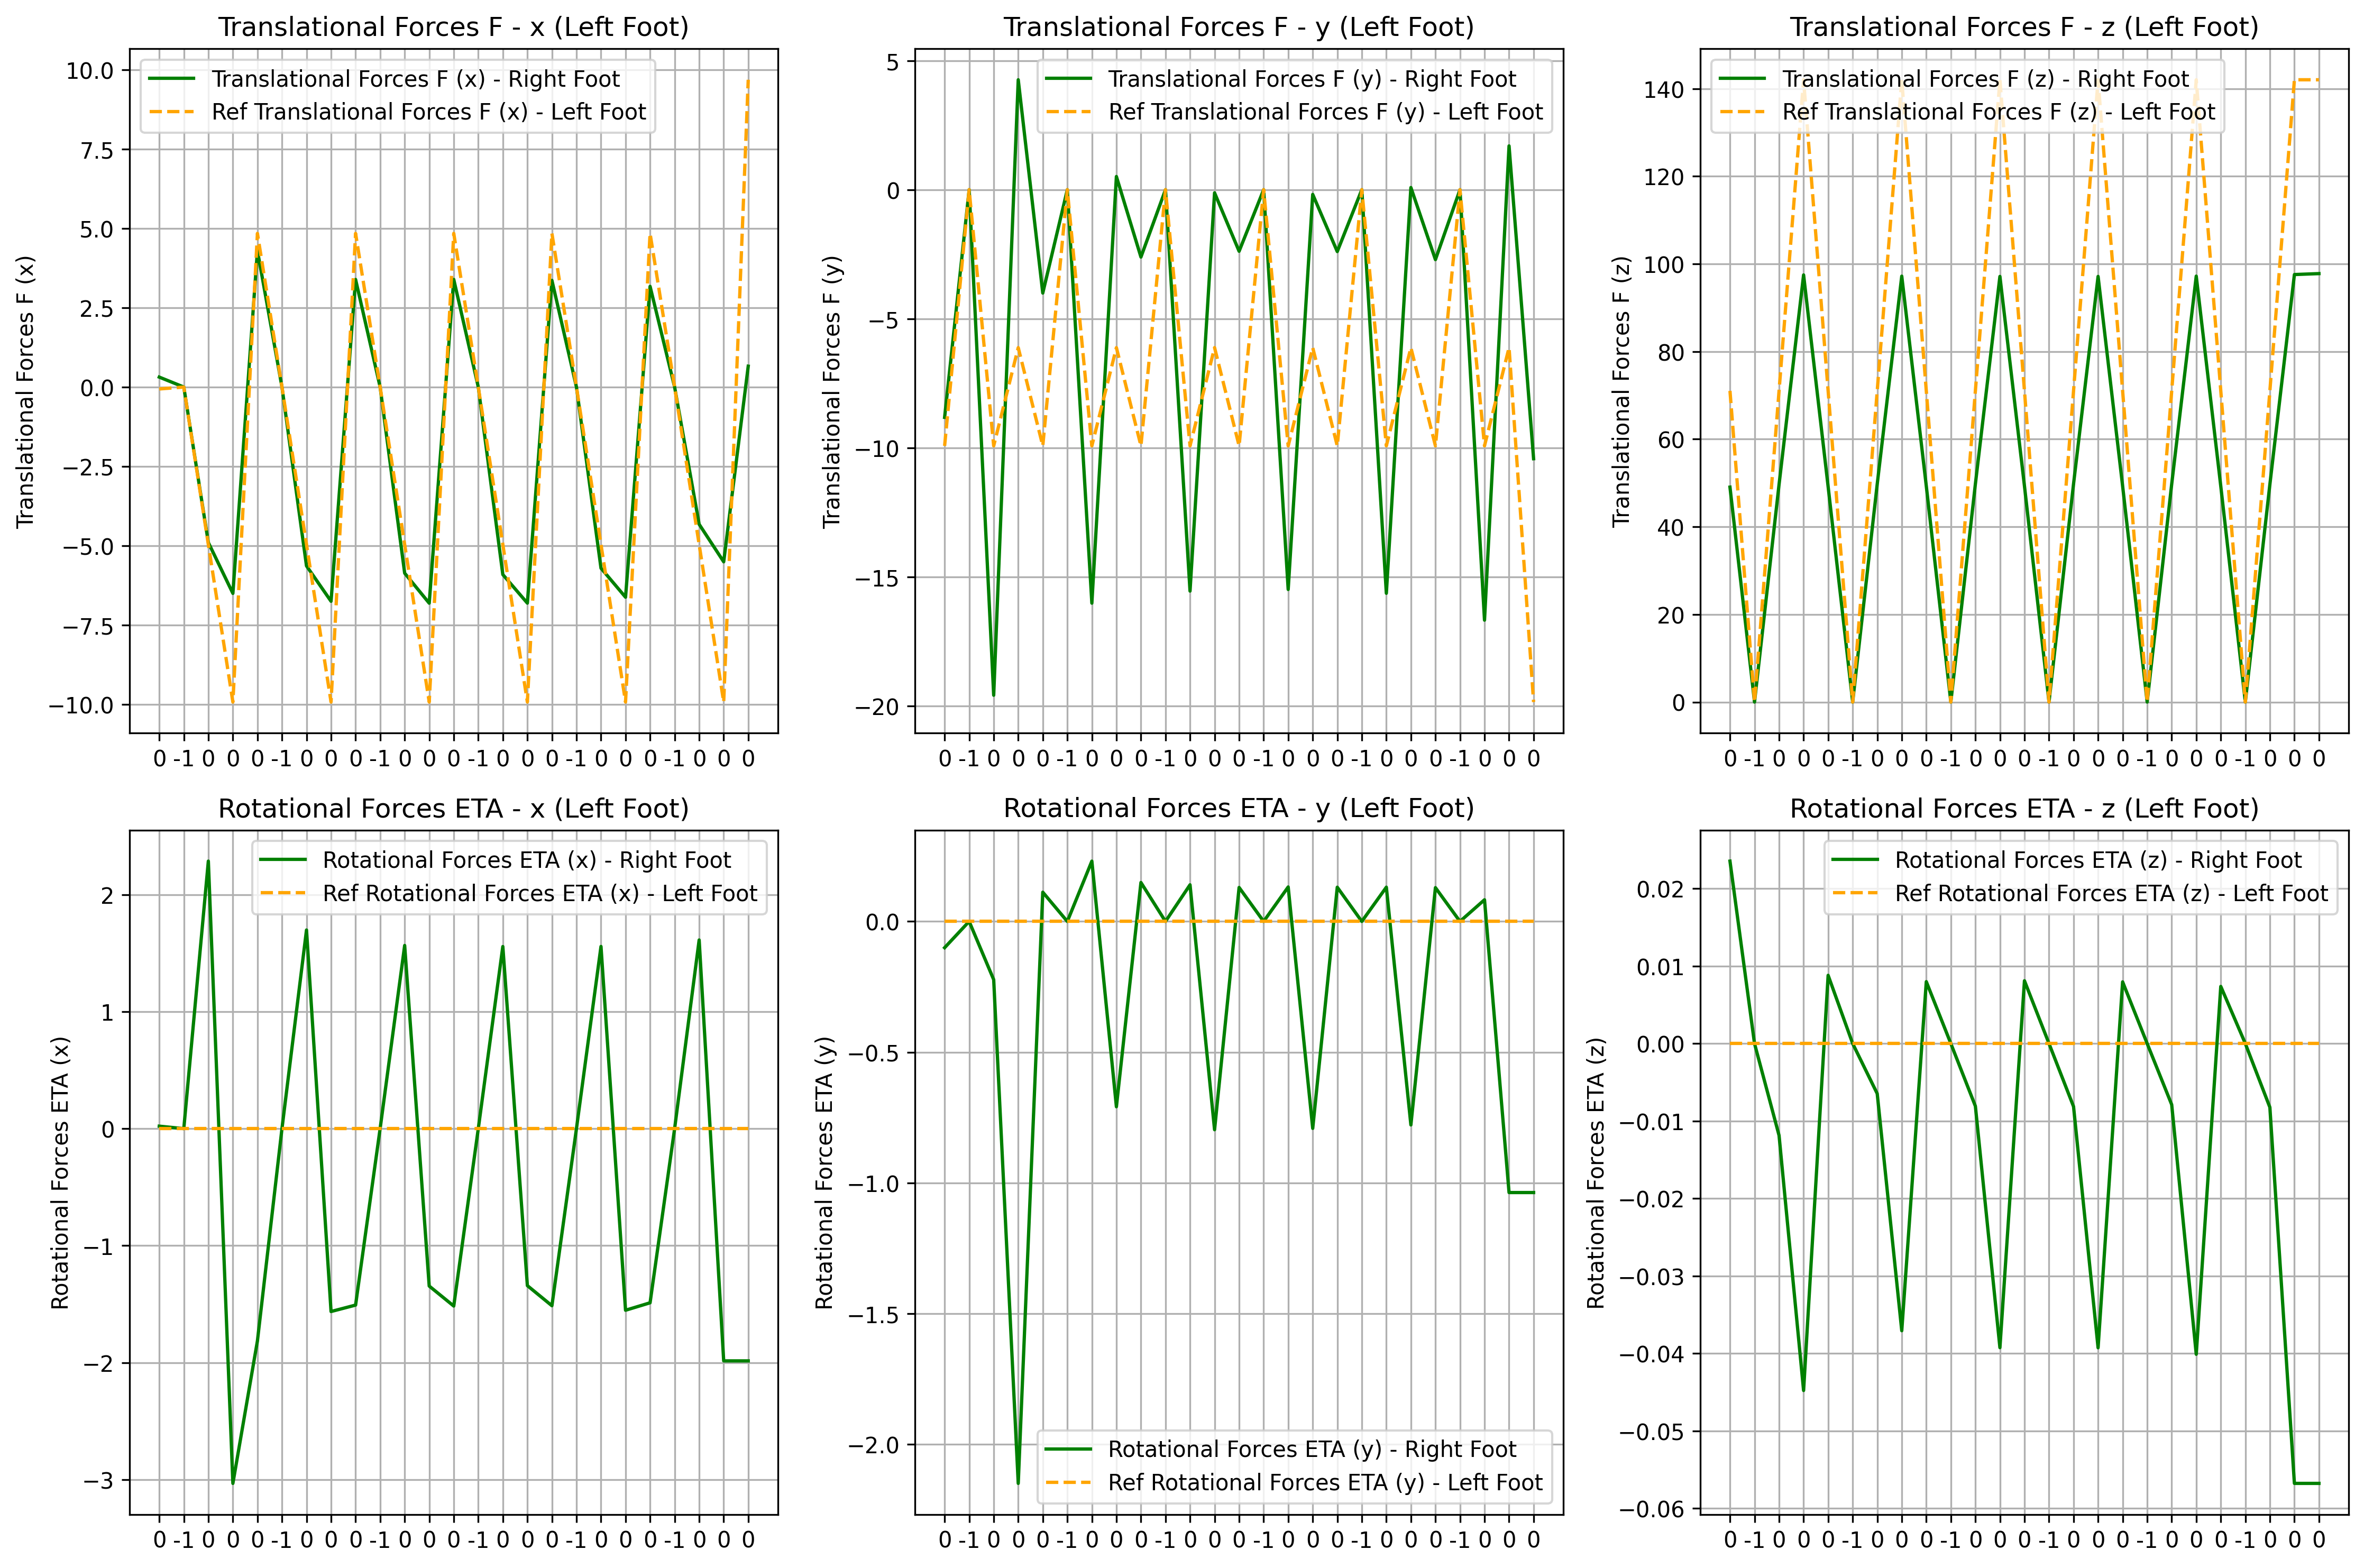
\includegraphics[width=0.8\textwidth]{figures/contact_forces_walking.png}
    \caption{Trajectory vs Reference: Forces}
    \label{fig:contact_forces_walking}
\end{figure}

\newpage
\subsubsection{Robot representation}
In this section it is possible to visualize first the path followed by the CoM, right and left foot in time:
\begin{figure}[htbp]
    \centering
    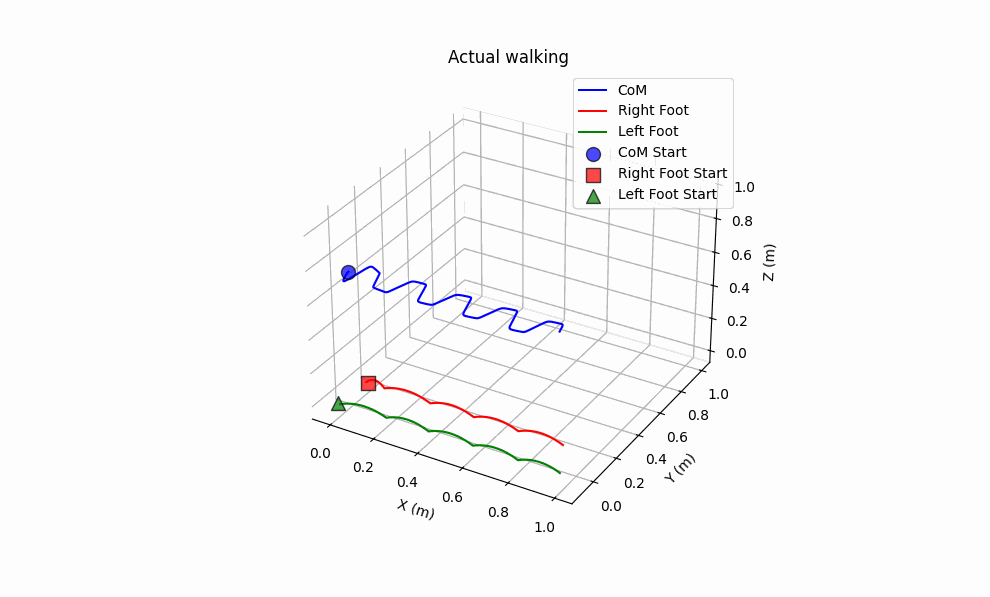
\includegraphics[width=0.8\textwidth]{figures/walking.PNG}
    \caption{Walking}
    \label{fig:walking}
\end{figure}

The CoM solution and reference foot are also passed to the URDF Skeleton into the Dart Simulation environment. 

\centering
\includemedia[
  width=0.8\linewidth,
  height=0.45\linewidth,
  activate=onclick,
  addresource=figures/walking_sim.mp4,
  flashvars={
     source=figures/walking_sim.mp4
    &autoPlay=true
  }
]{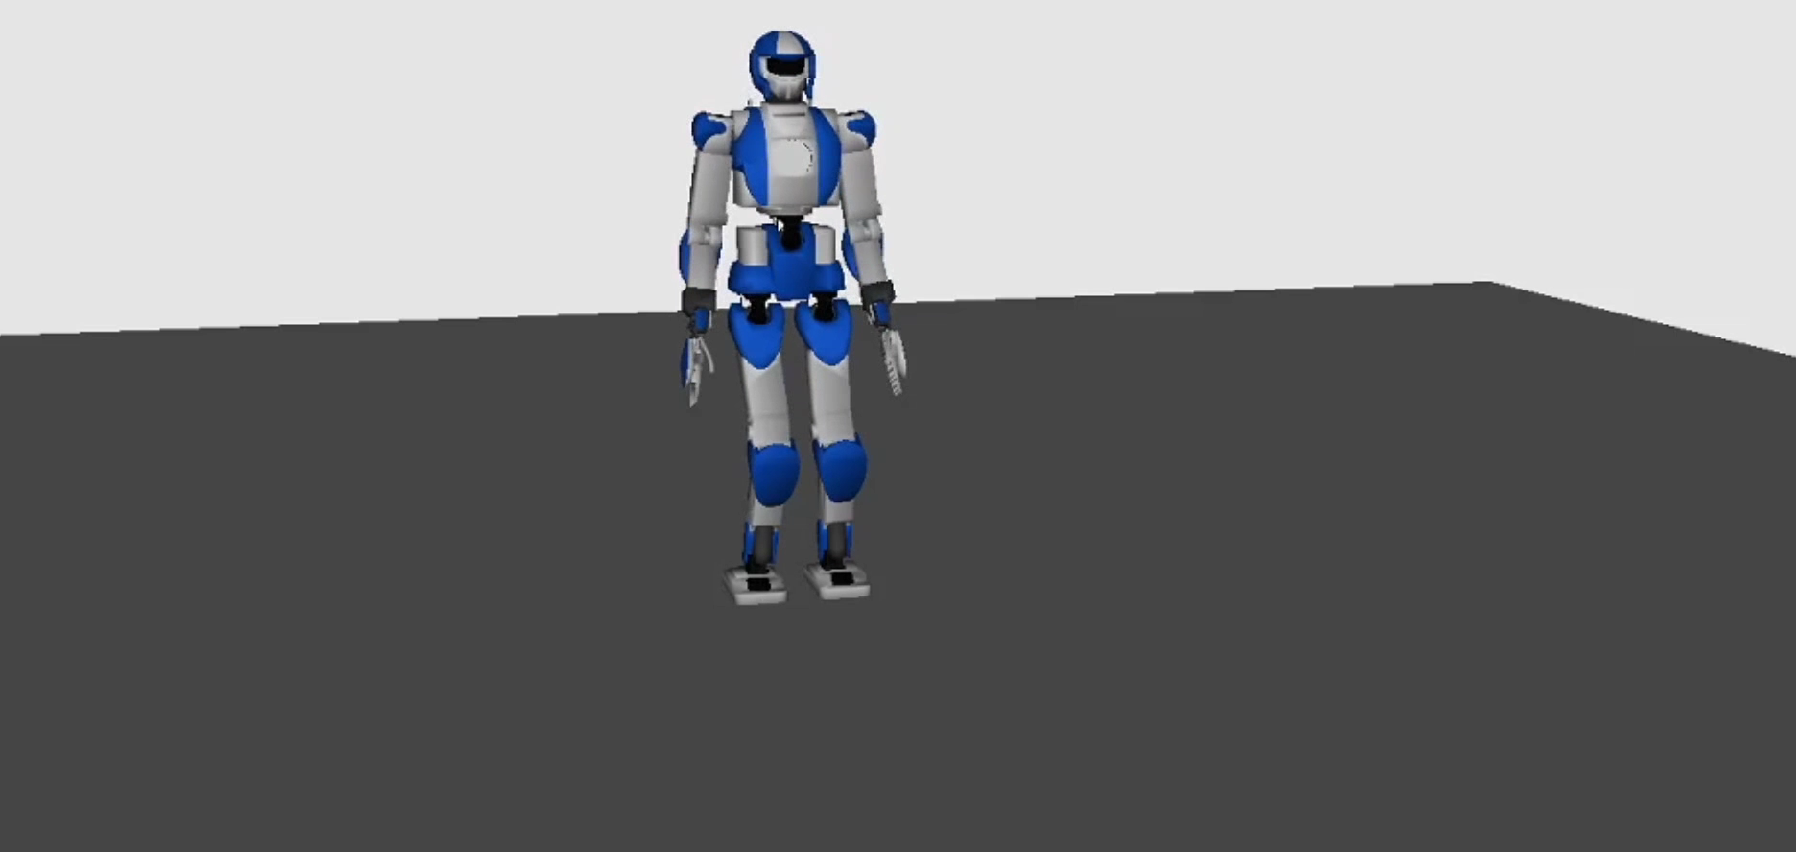
\includegraphics{figures/robot.PNG}}{VPlayer.swf}
 


\end{document}